Consider a database scheme of the form $S = (U, R, B)$, where $U$ is a set of database domains, $R$ is a set of database predicates or relations and $B$ is a set of finite built-in predicates.
For example, in this paper, $B = \{=, <, >, \neq, \leq, \geq, \approx\}$.
Let $Dom(A)$ be the domain of an attribute $A \in U$.
We denote by $I$ and instance of $S$ consisting of $n$ tuples.
Let $t$ be a single tuple from the instance $I$, we denote $t[A]$ or $I(t[A])$ the value of the cell of the tuple $t$ under attribute $A$.

The integrity constraints in this paper are identified by \textit{denial-constraints} over relational databases.
Denial constraints are first-order formulae of the form $ \varphi = \forall \overline{x}\neg(R_1(\overline{x_1}) \wedge ... \wedge R_n(\overline{x_n}) \wedge P_1 \wedge ... \wedge P_m)$,
where $R_i \in R$ is a relation atom, and $\overline{x} = \cup \overline{x_i}$, and each $P_i$ of the form $v_i \theta c$ or $v_i \theta v_j$, where $v_i, v_j \in \overline{x}$, $c$ is a constant,
and $\theta \in B$.
Similarity predicate $\approx$ is possitive when the edit distance between two strings is above a user-defined threshold $\delta$.
Note that sungle-tuple constraints, Functional Dependencies, Matching Dependencies and Conditional Functional Dependencies are special cases of 
unary and binary denial constraints with equality and similarity predicates.

For a given database instance $I$ of schema $S$ and a DC $\varphi$, if $I$ satisfies $\varphi$, we write $I \models \varphi$.
For a given set of DCs $\sum$, we say $I \models \sum$ if and only if $\forall \varphi \in \sum, I \models \varphi$.
A repair $I'$ of an inconsistent instance $I$ is an instance that satisfies $\sum$ and has the same set of tuple identifiers in $I$.
The values of attributes in $I'$ can be different from $I$.
Also, for attributes with infinite domains, there can be infinte number of possible repairs.
In cases of infinite domain attributes we represent the repairs using a variable that can accomodate \textit{fresh-value} for its domain.
A fresh value variable can have value from $Dom(A)/Dom^a(A)$, where $Dom^a(A)$ is the domain of the values for A which satisfy at least a predicate for each denial constraint involving \textit{fresh-value}.

Number of possible ways to get a repair $I'$ from $I$ are infinite.
Therefore, when sampling a repair $I'$ for an inconsistent instance $I$ it is crucial to filter the repairs that have minimal number of modifications.
A widely used criterion is the \textit{minimality of changes}.
In literature \cite{Bohannon,Kolahi,Chomicki,Greco,Beskales_sampling}, three main terms used to define minimality of changes are:
\textit{Cardinality-Minimal Repair, Cardinality-Set-Minimal Repair} and \textit{ Set-Minimal Repair}.
In \cite{Beskales_journal} these terms have been defined in context of FDs and CFDs.
We will show with the help of an example that these minimality definitions still hold in cases of Denial constraints with predicates in the set $B = \{=, <, >, \neq, \leq, \geq, \approx\}$.
Consider a database instance $I$ in table \ref{tab:eg3} and the following DC: $\varphi _1: \forall t_i,t_j \in R, \neg (t_i.A = t_j.A \wedge t_i.B > t_j.B \wedge t_i.C < t_j.C) $.
Figure \ref{fig:cardinalityEg} shows sample repairs and the repair space to which they belong.
Repair $I1$ in Fig. \ref{fig:cardinalityEg} is a cardinality-minimal repair because it has clearly the minimum number of changes to repair $I$, 
and is also a Cardinality-Set-Minimal and Set-Minimal repair, \cite{Beskales_journal} shows that Cardinality-Minimal is a subset of Cardinality-Set-Minimal space 
and Cardinality-Set-Minimal is a subset of Set-Minimal space.
Repair $I2$ is Not Cardinality-Minimal because it has more changes than $I1$, but it is still a Cardinality-SetMinimal and Set-Minimal.
Repair $I3$ is Not Cardinality-Set-Minimal and neither a Cardinality-Minimal repair, because the value of cell $t_2[C]$ can be changed back to 5 
and value of cell $t_3[C]$ and $t_4[C]$ can be changed to something else, say 6 and 7 respectively, and the repair still stays valid.
Repair $I4$ is Not Set-Minimal, because the values of cell $t_2[B]$ and $t_2[C]$ can be reverted to their original values 3 and 5 respectively, 
and the resulting instance will still be a valid repair of $I$.
\begin{table} \label{tab:eg3}
\centering 
\begin{tabular}{|c|c|c|c|}  \hline
      	 & A & B & C	\\ \hline
   $t_1$ & 1 & 8 & 9 	\\ \hline
   $t_2$ & 1 & 3 & 5  	\\ \hline
   $t_3$ & 1 & 4 & 2 	\\ \hline
   $t_4$ & 1 & 5 & 4 	\\ \hline
\end{tabular}
\caption{Inconsistent Instance I and DC $\varphi _1: \forall t_i,t_j \in R, \neg (t_i.A = t_j.A \wedge t_i.B > t_j.B \wedge t_i.C < t_j.C) $}
\end{table}

%\begin{table} \label{tab:eg3}
%\centering 
%\begin{tabular}{|c|c|c|c|}  \hline
%      	 & A & B & C	\\ \hline
%   $t_1$ & 1 & 8 & 9 	\\ \hline
%   $t_2$ & 1 & 3 & \cellcolor[gray]{0.9}1  	\\ \hline
%   $t_3$ & 1 & 4 & 2 	\\ \hline
%   $t_4$ & 1 & 5 & 4 	\\ \hline
%\end{tabular}
%\caption{Inconsistent Instance I and DC $\varphi _1: \forall t_i,t_j \in R, \neg (t_i.A = t_j.A \wedge t_i.B > t_j.B \wedge t_i.C < t_j.C) $}
%\end{table}
%
%\begin{table} \label{tab:eg3}
%\centering 
%\begin{tabular}{|c|c|c|c|}  \hline
%      	 & A & B & C	\\ \hline
%   $t_1$ & 1 & 8 & 9 	\\ \hline
%   $t_2$ & 1 & 3 & 5  	\\ \hline
%   $t_3$ & 1 & 4 & \cellcolor[gray]{0.9}7 	\\ \hline
%   $t_4$ & 1 & 5 & \cellcolor[gray]{0.9}8 	\\ \hline
%\end{tabular}
%\caption{Inconsistent Instance I and DC $\varphi _1: \forall t_i,t_j \in R, \neg (t_i.A = t_j.A \wedge t_i.B > t_j.B \wedge t_i.C < t_j.C) $}
%\end{table}
%
%\begin{table} \label{tab:eg3}
%\centering 
%\begin{tabular}{|c|c|c|c|}  \hline
%      	 & A & B & C	\\ \hline
%   $t_1$ & 1 & 8 & 9 	\\ \hline
%   $t_2$ & 1 & 3 & \cellcolor[gray]{0.9}3  	\\ \hline
%   $t_3$ & 1 & 4 & \cellcolor[gray]{0.9}4 	\\ \hline
%   $t_4$ & 1 & 5 & \cellcolor[gray]{0.9}5 	\\ \hline
%\end{tabular}
%\caption{Inconsistent Instance I and DC $\varphi _1: \forall t_i,t_j \in R, \neg (t_i.A = t_j.A \wedge t_i.B > t_j.B \wedge t_i.C < t_j.C) $}
%\end{table}
%
%\begin{table} \label{tab:eg3}
%\centering 
%\begin{tabular}{|c|c|c|c|}  \hline
%      	 & A & B & C	\\ \hline
%   $t_1$ & 1 & 8 & 9 	\\ \hline
%   $t_2$ & \cellcolor[gray]{0.9}2 & \cellcolor[gray]{0.9}6 & \cellcolor[gray]{0.9}7  	\\ \hline
%   $t_3$ & 1 & 4 & 2 	\\ \hline
%   $t_4$ & 1 & 5 & 4 	\\ \hline
%\end{tabular}
%\caption{Inconsistent Instance I and DC $\varphi _1: \forall t_i,t_j \in R, \neg (t_i.A = t_j.A \wedge t_i.B > t_j.B \wedge t_i.C < t_j.C) $}
%\end{table}
%

\begin{figure}
   \centering
   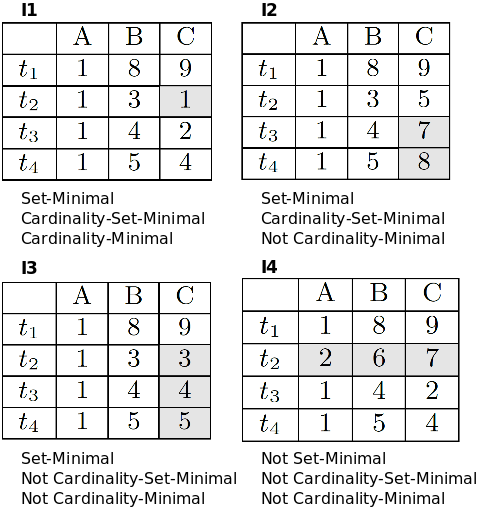
\includegraphics[scale=0.3]{cardinalityEg.png}
   \caption{Sample repairs from different repair space.}
   \label{fig:cardinalityEg}
\end{figure}
